\section{The Mozart Programming System}
In der vorliegenden Ausarbeitung soll das "`Mozart Programming System"'
\footnote{\url{http://www.mozart-oz.org}} 
vorgestellt werden. Bei \textsl{Mozart} handelt es sich um eine 
Programmierumgebung, die die multiparadigmische Programmiersprache \textsl{Oz} 
implementiert.

Entstanden ist Mozart-Oz ursprünglich als Forschungsprojekt am Deutschen 
Forschungszentrum für Künstliche Intelligenz (DFKI) sowie der Universität 
Saarbrücken. Inzwischen wird die Sprache vom Mozart-Konsortium, zu welchem 
Arbeitsgruppen aus Belgien, Schweden und Deutschland gehören, weiterentwickelt. 
Die Quellen sind unter einer Open-Source-Lizenz verfügbar; ein kommerzieller 
Einsatz der Sprache ist ebenfalls möglich.

Ähnlich wie in Java können Oz-Programme in eine Art Byte-Code übersetzt werden 
und laufen anschließend in einer virtuellen Maschine ab. Auf diese Weise wird 
eine gewisse Plattformunabhängigkeit erreicht.

\section{Die Programmiersprache Oz}
\subsection{Features}
Als Hauptfeatures und -vorteile von Oz gelten die folgenden Aspekte:

\begin{description}
  \item[Nebenläufigkeit] Arbeit mit leichtgewichtigen Threads, 
  Datenfluss-Synchronisation.
  \item[Inferencing] Constraintbasierte und 
  logische Programmierung.
  \item[Verteilung] Transparente 
  Netzwerkunterstützung.
  \item[Flexibilität] Dynamische Typisierung, inkrementelles 
  Kompilieren.
\end{description}

\subsection{Datentypen}
Die Sprache stellt eine Reihe von Datentypen zur Verfügung, deren Hierarchie in 
Abbildung \ref{fig:oz-datentypen} dargestellt ist.

\begin{figure}[hp]
  \centering 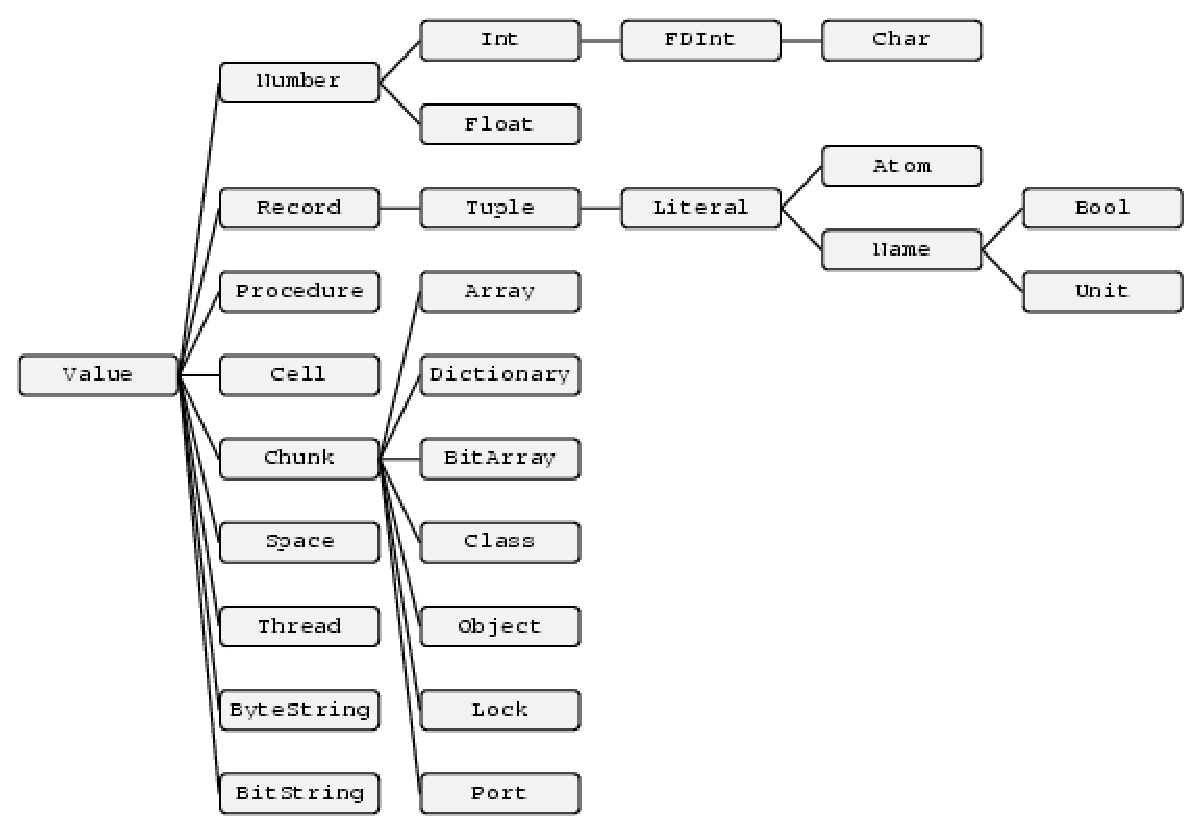
\includegraphics[width=0.70\textwidth]{../images/oz-datentypen} 
  \caption{Hierarchie der Datentypen in Oz 3. Quelle:
  \cite[Tutorial of Oz, Chapter 3.1]{url:mozart-documentation}}
  \label{fig:oz-datentypen}
\end{figure}

Einige der wichtigsten Datentypen seien hier kurz aufgeführt (vgl. 
\cite{Brunklaus:00}).

\begin{enumerate}
  \item Einfache Werte
    \begin{description}
      \item [Zahlen] können in Oz sowohl als ganze Zahlen (\texttt{Int, Char})
      als auch Fließkommazahlen (\texttt{Float}) benutzt werden.
      \item[Literale] teilen sich auf in sog. Atome und Namen. Ein Atom wird 
      durch eine alphanumerische Zeichenkette beschrieben, die entweder mit 
      einem Kleinbuchstaben beginnt oder in Hochkomma gefasst ist. Namen sind 
      eindeutige Bezeichner, die über eine spezielle Prozedur namens 
      \texttt{NewName} erzeugt werden können.
      \item[Prozeduren] können in Oz an Variablen gebunden und auch zur 
      Laufzeit erzeugt werden. \end{description}
  \item Zusammengesetzte Werte
    \begin{description}
      \item[Records] bestehen aus einem Bezeichner (Label) sowie einer festen 
      Anzahl von Komponenten oder Argumenten. Argumente bestehen aus dem Tupel 
      (Feature, Feld).
      \item[Tupel] sind ein Spezialfall von Records, bei denen die Argumente 
      kein explizites Feature besitzen.
      \item[Listen] sind eine Sonderform der Tupel. Die leere Liste wird mit
      \texttt{nil} denotiert, offene Listen bspw. als \texttt{1|2|3|nil} und 
      geschlossene Listen (also Listen mit fester Elementanzahl) als \texttt{[1 
      2 3]}.
    \end{description}
  \item \textbf{Chunks} erlauben es, abstrakte Datentypen zu konstruieren. 
  Oz bringt bereits einige vordefinierte Chunks mit, z.B. \texttt{Array} 
  oder \texttt{Dictionary}.
\end{enumerate}

\subsection{Multiparadigmisch?}
Wie bereits eingangs erwähnt, unterstützt Oz mehrere Programmierparadigmen:

\begin{enumerate}
  \item Constraint-Programmierung
  \item Funktionale Programmierung
  \item Objektorientierte Programmierung
  \item Logische Programmierung
\end{enumerate}
  
Im Gegensatz zu einer Programmiersprache, die nur eines der Paradigmen 
unterstützt, lassen sich in Oz also die zu lösenden Probleme von mehreren 
Seiten gleichzeitig mit dem jeweils geeignetsten Paradigma bearbeiten. 
Erreichen könnte man dies zwar auch durch die Kombination verschiedener 
Programmiersprachen, dabei bliebe aber der Nachteil, dass man semantische 
Lücken überwinden und Schnittstellen zwischen den einzelnen Sprachen definieren 
müsste. Dies würde u.a. zu einer aufwendigeren Fehlersuche führen. Mit Oz 
lassen sich hingegen die verschiedene Paradigmen problemlos miteinander 
kombinieren, deren gemeinsame Basis, das Oz Programming Model, im nächsten 
Abschnitt vorgestellt wird.

\subsection{Programmiermodell (Oz Programming Model, OPM)}
Die Grundlage für Berechnungen in Oz bildet das so genannte \textsl{Concurrent 
Constraint Programming}. Alle weiteren Paradigmen werden durch sog. "`syntactic 
sugar"' (Syntaxerweiterungen) in die Sprache integriert \cite{KI-LP96}.

Allgemein verwendet das Modell für Berechnungen die Metapher eines sog. 
\textsl{Berechnungsraums} (Computational Space). In diesem befindet sich zum 
einen ein \textsl{Speicher}, zum anderen eine Anzahl von sog. \textsl{Aktoren}. 
Aktoren führen die eigentlich Berechnung durch, indem sie schrittweise 
reduziert werden und sich dabei über den gemeinsamen Speicher synchronisieren. 
Dazu können Aktoren Information in den Speicher schreiben (tell) und auf 
Information warten und diese anfordern (ask).

Nebenläufigkeit (Concurrency) ist einer der wichtigsten Aspekte des OPM. Dabei 
bedeutet Nebenläufigkeit, dass verschiedene Berechnungen unabhängig voneinander 
durchgeführt werden können, nicht, dass diese parallel ablaufen.
